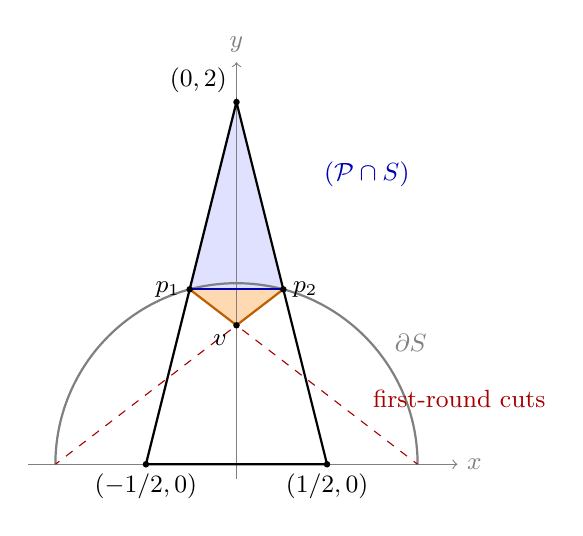
\begin{tikzpicture}[scale=2.3, every node/.style={font=\small}]
 \pgfmathsetmacro{\contactt}{(1+2*sqrt(13))/17}
 \pgfmathsetmacro{\contactx}{(1-\contactt)/2}
 \pgfmathsetmacro{\contacty}{2*\contactt}
 \pgfmathsetmacro{\closurey}{(1+sqrt(13))/6}
 \coordinate (top) at (0,2);
 \coordinate (left) at (-.5,0);
 \coordinate (right) at (.5,0);
 \coordinate (p1) at (-\contactx,\contacty);
 \coordinate (p2) at (\contactx,\contacty);
 \coordinate (v) at (0,\closurey);
 \fill[blue!12] (top)--(p1)--(p2)--cycle;
 \fill[orange!30] (p1)--(v)--(p2)--cycle;
 \draw[gray,thin,->] (-1.15,0)--(1.22,0) node[right] {$x$};
 \draw[gray,thin,->] (0,-.08)--(0,2.22) node[above] {$y$};
 \draw[gray,thick] (1,0) arc[start angle=0,end angle=180,radius=1];
 \draw[black,thick] (top)--(left)--(right)--cycle;
 \draw[red!65!black,dashed] (p1)--(1,0);
 \draw[red!65!black,dashed] (p2)--(-1,0);
 \draw[blue!70!black,thick] (p1)--(p2);
 \draw[orange!75!black,thick] (p1)--(v)--(p2);
 \foreach \point in {top,left,right,p1,p2,v}
   \fill (\point) circle[radius=.018];
 \node[above left] at (top) {$(0,2)$};
 \node[below] at (left) {$(-1/2,0)$};
 \node[below] at (right) {$(1/2,0)$};
 \node[left] at (p1) {$p_1$};
 \node[right] at (p2) {$p_2$};
 \node[below left] at (v) {$v$};
 \node[gray,above right] at (.82,.57) {$\partial S$};
 \node[blue!70!black,align=left,right] at (.43,1.6)
   {$\conv(\mathcal P\cap S)$};
 \node[red!65!black,align=left,right] at (.7,.36)
   {first-round cuts};
\end{tikzpicture}
